\documentclass{article}
\usepackage{spconf,amsmath,graphicx}

\usepackage{color}
\usepackage{balance}
\linespread{1}
\usepackage{dblfloatfix}

\def\x{{\mathbf x}}
\def\L{{\cal L}}

% Title.
% ------
\title{Measuring Thickness profile between closed curves applied to
  endometritis detection in cattle}

% \name{Mat\'ias Tailani\'an, Federico Lecumberry, Alicia Fern\'andez, Gregory Randall, }
% \address{Facultad de Ingenier\'ia, Universidad de la Rep\'ublica\\
% 	 Julio Herrera y Reissig 565, Montevideo, Uruguay}

\twoauthors
 {M. Tailani\'an, A. Fern\'andez, F. Lecumberry }%, G. Randall}
	{Facultad de Ingenier\'ia, Universidad de la Rep\'ublica\\
	 Julio Herrera y Reissig 565, Montevideo, Uruguay}
 {G. Gnemmi}
	{Bovinevet\\
	 Premosello Chiovenda (VB), Italy}

\begin{document}
\maketitle

\begin{abstract}
In this paper we address the problem of defining and measuring a thickness profile between closed curves that do not intersect and one is interior to the other. Based on the normal evolution of curves, we developed an algorithm that defines the correspondence between points of different curves and measures the thickness profile. Ensuring in each step a good sampling of all curves by of creating and combining points, the algorithm splits the evolution in two parts, evolving from the convex hull of the interior curve to each one of the others. The thickness profile obtained is used to extract some features to detect a uterine disease (endometritis) in dairy cattle, based in ultrasound images. Some results of thickness profiles in real and sythetic curves are shown, as well as a preliminary endometritis diagnose using this features. 
\end{abstract}

\begin{keywords}
Curves evolution, thickness, distance, endometritis, ultrasound images.
\end{keywords}

\section{Introduction}
\label{sec:intro}
Given two closed curves, that do not intersect and one is interior to the other, this work addresses the problem of finding an entire thickness profile between them. Figure \ref{fig:defs}a shows a typical setting of the curves involved in the problem: $\Gamma_1$, $\Gamma_2$, $\Gamma_3$. None of the curves is assumed to be convex, but typically $\Gamma_1$ and $\Gamma_2$ presents a smooth curvature variation, while $\Gamma_3$ (typically non convex) presents a high curvature variation and in some cases is even not differentiable in some points. 
\begin{figure}[t]
\begin{minipage}[b]{.45\linewidth}
  \centering
  \centerline{
\includegraphics[width=3.8cm]{pics/defs2}}
  \centerline{(a)}\medskip
\end{minipage}\hfill
\begin{minipage}[b]{.52\linewidth}
  \centering
  \centerline{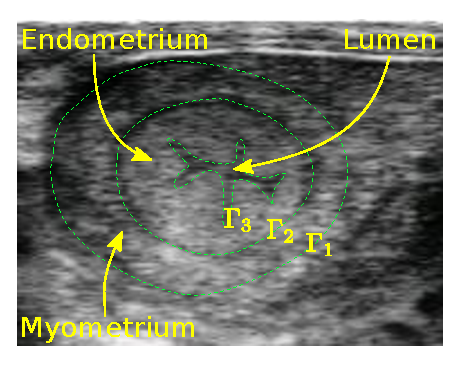
\includegraphics[width=4.2cm]{pics/defsEndo}}
  \centerline{(b)}\medskip
\end{minipage}
\vspace{-10pt}
\caption{Definitions. A schematic representation of the problem is shown in (a), while in (b) is presented a real example of the application. The region between $\Gamma_1$ and $\Gamma_2$ is called \emph{Myometrium}, the region between $\Gamma_2$ and $\Gamma_3$ \emph{Endometrium} and the region inside $\Gamma_3$ \emph{Lumen}.}
\vspace{-5pt}
\label{fig:defs}
\end{figure}
The main goal is to define and measure the thickness profile of the regions between $\Gamma_1$ and $\Gamma_2$, and between $\Gamma_2$ and $\Gamma_3$.

In the literature there are some measures of distance between two curves, such as Housedorff~\cite{libroMorel}, or Sobolev~\cite{statistics}, providing a numeric value for the distance or dissimilarity between curves, but we are interested, as said, in the entire thickness profile. To compute the thickness of a region, the first question to ask is how to conceptually define the thickness between two curves. Several methods, like the one presented in~\cite{paperWarping}, finds the correspondence between two morphologically different objects by the minimization of a similarity criterion function. Other methods resolve the correspondence by circle mapping~\cite{libro}: the vertices of the origin and target curves are projected on circles of the same radius, and then merged. The merged set of vertices are projected back onto each curve, obtaining curves with the same number of vertices, and in a pairwise correspondence. In this work we propose a simple algorithm that finds this correspondence in a natural way using curves evolution \cite{curvesEvol}. It is based on the normal evolution of the interior curve (the origin curve) and considers the other curve as target. In the evolution are included some mechanisms of creating and combining points to ensure a correct sampling at all steps. The thickness is measured as the length of the path in the evolution. This algorithm finds an intuitive correspondence between points of the different curves and leads to an appropriate thickness definition.

The application considered is to detect a common uterine disease (endometritis) in dairy cattle using ultrasound (US) images. The relation between some muscles thickness can be a relevant feature to diagnose this disease~\cite{Gianni2010}, so in this work we explore this possibility developing a system to measure this feature. In Figure \ref{fig:defs}b is shown a typical US image with the curves $\Gamma_i,\;\;i=1\dots3$ overprinted. Curves are always in this order and there is no intersection between them, since they are the limits of muscles and tissues in cattle uterine horns. Measuring the thickness profile of the Myometrium and Endometrium is the goal of this work.
\begin{figure*}[t]
\begin{minipage}[b]{.32\linewidth}
  \centering
  \centerline{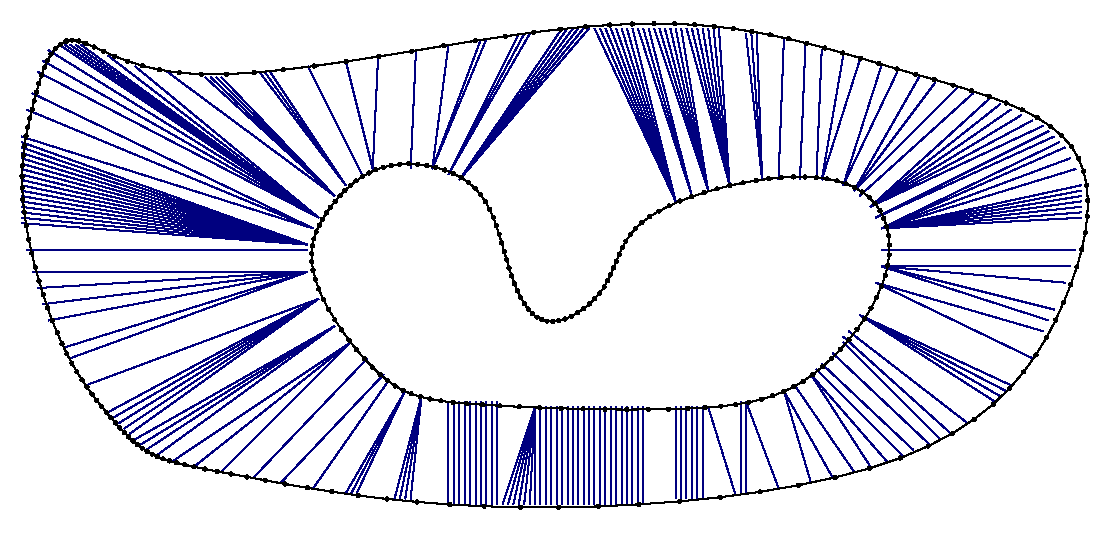
\includegraphics[width=5.8cm]{pics/cmp_dist}}
  \centerline{(a)}\medskip
\end{minipage}
\hfill
\begin{minipage}[b]{.32\linewidth}
  \centering
  \centerline{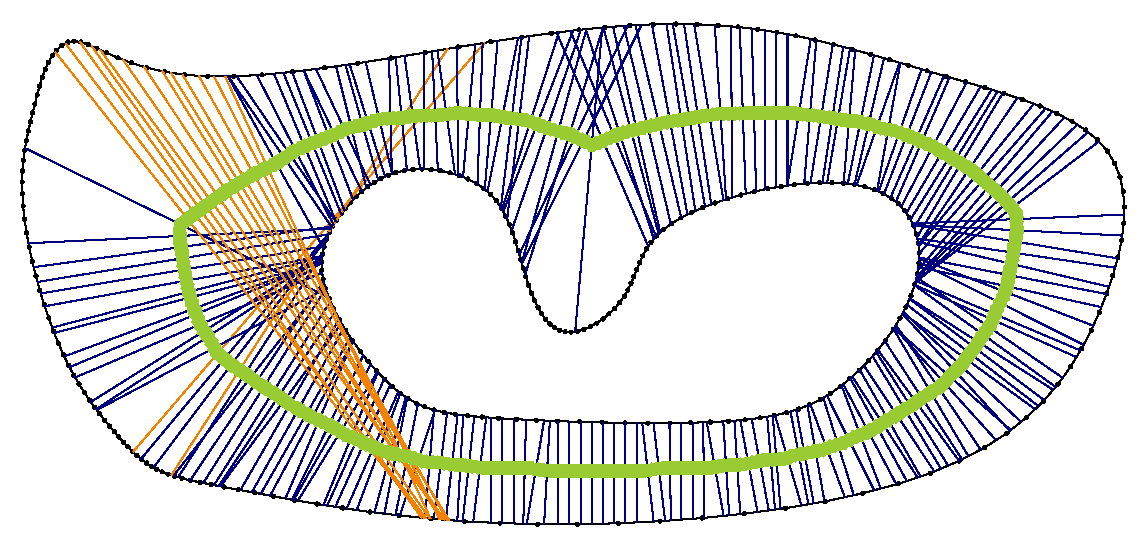
\includegraphics[width=5.8cm]{pics/cmp_norm2}}
  \centerline{(b)}\medskip
\end{minipage}
\hfill
\begin{minipage}[b]{.32\linewidth}
  \centering
  \centerline{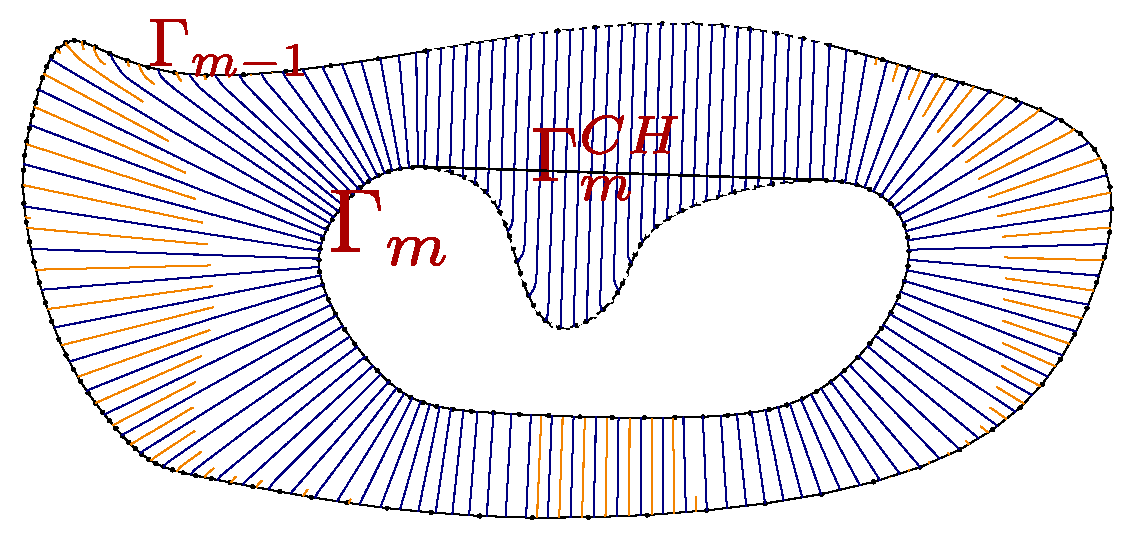
\includegraphics[width=5.8cm]{pics/cmp_evol_pelada}}
  \centerline{(c)}\medskip
\end{minipage}
\caption{Comparison between different proposals. (a) Distance function from the points in the outer curve to the inner curve. (b) Defining the middle curve as the curve equidistant to both curves, the thickness is measured as the length of the normal to the middle curve. (c) Proposal: the blue lines represent the path traveled by the original points during evolution, and the orange lines corresponds to points created during evolution, see Section \ref{sec:proposal}.}
\label{fig:comp}
\vspace{-10pt}
\end{figure*}

The description of the particular problem considered and the proposal are presented in Section \ref{sec:proposal}. In Section \ref{sec:results} are presented results using synthetic and real curves and a final application to diagnose endometritis using descriptors extracted from the thickness profile. Finally, in Section \ref{sec:conc} we present conclusions and future work.


\section{Problem description and proposal}
\label{sec:proposal}

\subsection{Problem description}
\label{ssec:description}
In order to understand the particular application considered it is important to define some concepts. In Figure \ref{fig:defs}b a transverse cut of cattle uterine horn is shown. We can imagine the uterine horn as a tube with two coatings: Endometrium and Myometrium. The Myometrium is the region delimited by $\Gamma_1$ and $\Gamma_2$ and the Endometrium is the region delimited by $\Gamma_2$ and $\Gamma_3$. The problem is to measure the thickness of those two regions, using a manual segmentation of the regions.
While searching for a definition of the distance between two curves, euclidean distance comes to head. In this case, for each point of curve $\Gamma_i$ the nearest point of $\Gamma_j$ is found and the euclidean distance between this two points is used as thickness. As can be seen in Figure \ref{fig:comp}a, this thickness definition cannot capture the curves ``structure'', deriving in a wrong profile. Another idea is to measure width in the normal direction of each point of the curve. Considering the normal to curve $\Gamma_2$, we cannot ensure that this direction will intersect $\Gamma_3$. With the purpose of obtaining a more regular curve and define the thickness in the normal direction of this new curve, we consider the skeleton of the region defined by $\Gamma_2$ and $\Gamma_3$, defined as the curve $\Gamma_{23}$ equidistant to both curves. The results of measuring the thickness in the normal direction of each point of $\Gamma_{23}$ are not as expected and in some directions the normals do not intersect curve $\Gamma_3$ (See Figure \ref{fig:comp}b). Finally, in Figure \ref{fig:comp}c is presented our proposed algorithm. In this case, the ``structure'' of the curves are effectively captured, obtaining a distance between curves that can be interpreted as thickness.

Another possibility is to create synthetic images from the given curves in order to use other methods like GAC \cite{gac} o Chan-Vese \cite{chan-vese}, that uses image data to perform the evolution. However, this methods introduce other terms representing for example the curve regularity or area measures that are not linked to the original problem and may hinder the real problem of measuring a region thickness. 

\subsection{Proposal}
\label{ssec:proposal}
Our proposal is based on the simplest curves evolution: the normal evolution. Letting $\eta$ be the evolution step and $\vec{n}_{p_i}^t$ the normal to the curve at the point $p_i$ at time $t$, the evolution is governed by the equation:
\begin{equation}
  p_i^{t+1}=p_i^t+\eta \; \vec{n}_{p_i}^t.
  \label{ec:normal}
\end{equation}
Due to the nature of the curves described in Section \ref{sec:intro}, considering the non convexity of the curves, we propose to perform a two step evolution, which in the final step are joined to obtain a single result. While measuring the thickness between $\Gamma_m$ and $\Gamma_{m-1}$, if $\Gamma_m$ is non convex, an auxiliary curve is considered: the convex hull of curve $\Gamma_m$ ($\Gamma_m^{CH}$) ~\cite{libro}. The two steps of the evolution are: 1) Evolution from $\Gamma_m^{CH}$ to $\Gamma_m$, and 2) Evolution from $\Gamma_m^{CH}$ to $\Gamma_{m-1}$. The final width, or distance between curves, is calculated as the distance of the path traveled by each point of the curve. The original curves are created with a cubic interpolation of a few points indicated by the expert and then re-sampled according to curvature, using more points in regions with higher curvature. The sampling of $\Gamma_m^{CH}$ is done by two different ways according to each point nature: points $p_i\in\Gamma_{m}$ that also belongs to $\Gamma_m^{CH}$ are directly used, and in regions where $\Gamma_m$ do not match $\Gamma_m^{CH}$, an uniform sampling is performed such that both curves have the same number of points.

Sampling conditions are considered at each step to ensure a correct representation of the curve. For that purpose we developed a simple mechanism of creating and combining points while evolving the curve. At the beginning of the evolution, the mean distance, $\delta$, between adjacent points is computed. The procedure of creating new points consists on evaluating at each evolution step $t$ if the distance between two adjacent points $p_i^t$ and $p_{i+1}^t$ is greater than $2\delta$. In this case, a new point, $p_k^t$, is created between $p_i^t$ and $p_{i+1}^t$ as the middle point. $p_k^t$ is initialized with the mean of the distance traveled by points $p_i^t$ and $p_{i+1}^t$, see Figure \ref{fig:nacimiento_y_muerte}a. The procedure to combine points is based on the evaluation of a proximity condition. If $\eta\frac{\vec{n}_{p_i}^{t-1}}{||\vec{n}_{p_i}^{t-1}||}$ and $\eta\frac{\vec{n}_{p_i+1}^{t-1}}{||\vec{n}_{p_i+1}^{t-1}||}$ are intersected, points $p_i^t$ and $p_{i+1}^t$ will be joined into a new one, placed in that intersection, see Figure \ref{fig:nacimiento_y_muerte}b.
\begin{figure}[t]
\begin{minipage}[b]{.5\linewidth}
  \centering
  \centerline{
\includegraphics[width=4.3cm]{pics/nacimiento}}
  \centerline{(a)}\medskip
\end{minipage}
\hfill
\begin{minipage}[b]{.48\linewidth}
  \centering
  \centerline{
\includegraphics[width=3.7cm]{pics/muerte}}
  \centerline{(b)}\medskip
\end{minipage}
\caption{Mechanisms of creating and combining points during evolution. (a) A new point is created (red point) if the distance between adjacent points exceeds a predefined threshold. (b) Two points are combined if their normals normalized and multiplied by the step length intersect each other.}
\label{fig:nacimiento_y_muerte}
\end{figure}
%If the curvature of curve $\Gamma_2$ is very high, the procedure should change a little, considering the convex hull of $\Gamma_2$ and perfoming the same procedure as the described for $\Gamma_3$.
% tengo que decir como se mide la normal: con un vecino de cada lado.

\section{Experiments and results}
\label{sec:results}
\subsection{Synthetic}
\label{ssec:syn}
In order to show the algorithm performance, a synthetic example is presented. This example was designed considering $\Gamma_i$, $i=1\dots3$ as three concentric circles and adding a perturbation in $\Gamma_2$ and $\Gamma_3$. This perturbations are introduced by adding in the normal direction of each point of the curve a Gaussian distribution $X \sim \mathcal{N}(0,1)$ centered in points with null phase for $\Gamma_2$ and centered in the points with maximum (absolute) phase for $\Gamma_3$. In the point where $X$ is maximal, the width of the region delimited by $\Gamma_1$ and $\Gamma_2$ is equal to the width of the region delimited by $\Gamma_2$ and $\Gamma_3$. The results are shown in Figure \ref{fig:synth}. Figure \ref{fig:synth}a shows the trajectory of the points while evolving. The trajectory of the original points is represented in blue color, while the trajectory of points created during evolution is represented in orange color. Figure \ref{fig:synth}b shows the thickness profile obtained relative to the angle measured from the center of the circles. As can be seen, the results are as expected. Near points with null phase, region between $\Gamma_1$ and $\Gamma_2$ presents a thickness decay while the region between $\Gamma_2$ and $\Gamma_3$ shows an increase. For the points with null phase and the points with maximal (absolute) phase the widths are equal. 
\begin{figure}[t]
\begin{minipage}[b]{1\linewidth}
  \centering
  \centerline{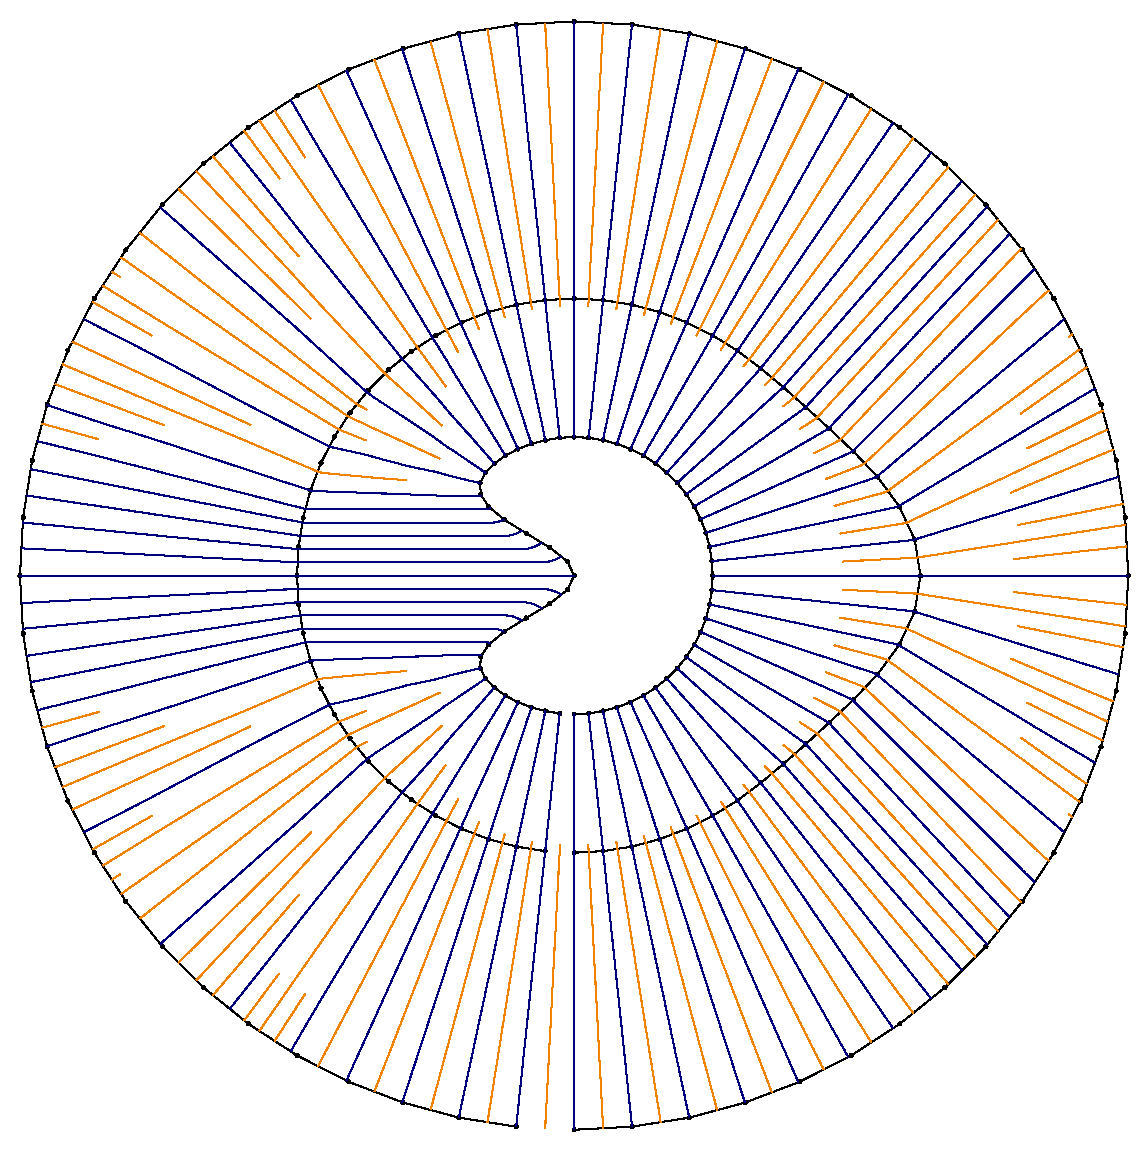
\includegraphics[width=5cm]{pics/synth4}}
  \centerline{(a)}\medskip
\end{minipage}
\begin{minipage}[b]{1\linewidth}
  \centering
  \centerline{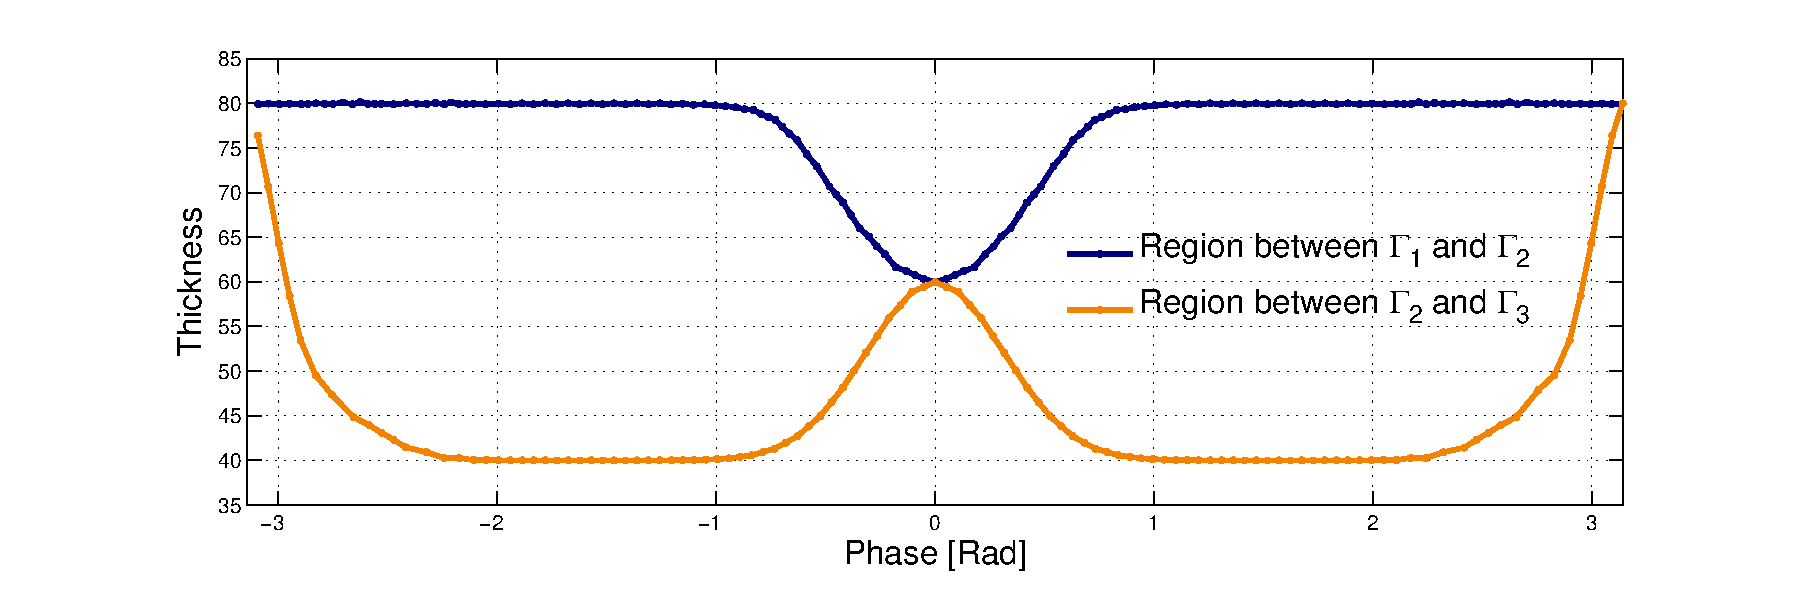
\includegraphics[width=8.5cm]{pics/synthWidth4}}
  \centerline{(b)}\medskip
\end{minipage}
\caption{Creation and combination of curve points. (a) Path traveled by points during the evolution. The blue lines corresponds to the evolution of the original points, while orange lines corresponds to created points. (b) Thickness profile relative to the angle measured from the center of the circles. In blue is shown the thickness of region between $\Gamma_1$ and $\Gamma_2$, and in orange between $\Gamma_2$ and $\Gamma_3$.}
\label{fig:synth}
\end{figure}

\subsection{Real}
\label{ssec:real}
Postpartum uterine diseases, such as endometrium damage and ovarian cyclic activity disruption, has become one of the most important causes of reproductive inefficiency in dairy cattle and are associated with infertility \cite{sheldon2008,barlund2008}. Endometritis is an uterine disease defined as inflammation limited to the endometrium occurring at least 21 days after calving and not associated with systemic illness \cite{sheldon2010}. This disease do not always presents clinical symptoms, so sub-clinical Endometritis detection using ultrasonography images is used \cite{Gianni2010, Gianni2013}. The sub-clinical endometritis diagnostic is very difficult, even for an expert, so image processing techniques to aid veterinaries in diagnostics get special relevance.

In this section we present results obtained in real ultrasonography images. The curves were manually segmented by the expert and our algorithm applied to obtain the thickness profile. Results are shown in Figure \ref{fig:real} for three real examples.

\begin{figure*}[t]
\begin{minipage}[b]{.26\linewidth}
  \centering
  \centerline{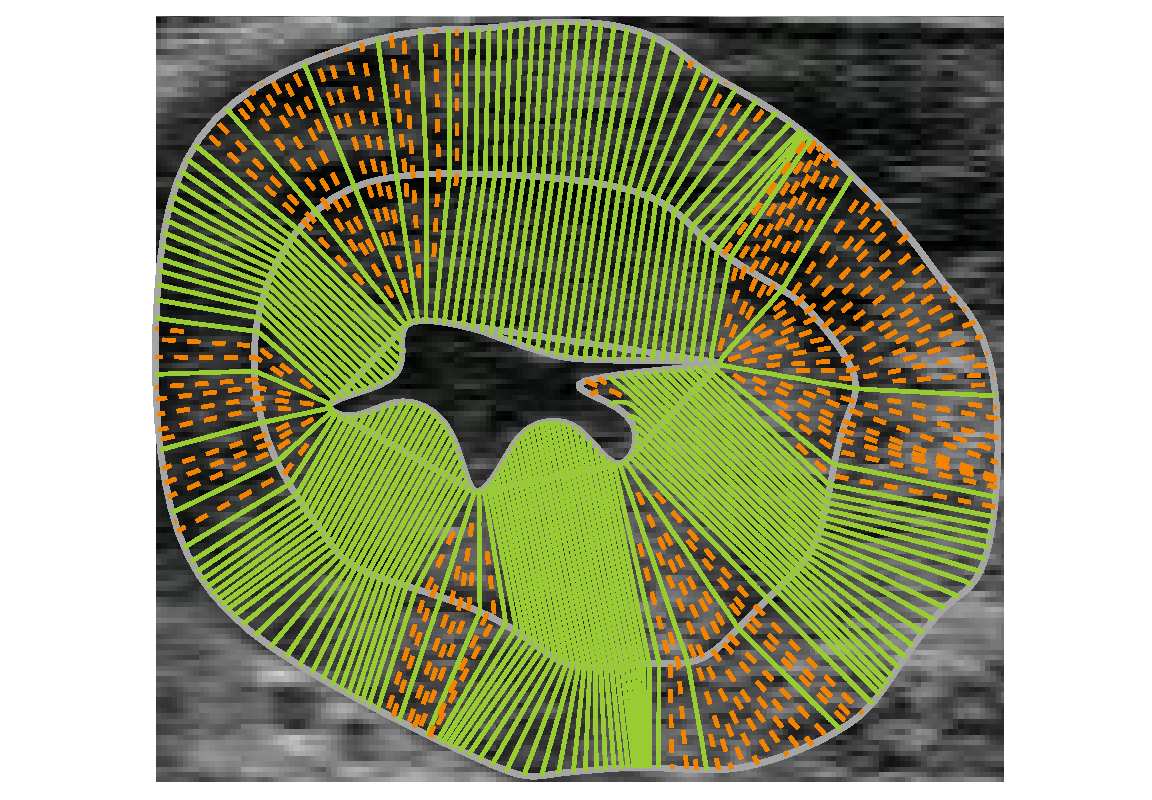
\includegraphics[width=6.25cm]{pics/rreal}}
  \centerline{(a)}\medskip
\end{minipage}
\hfill
\begin{minipage}[b]{.33\linewidth}
  \centering
  \centerline{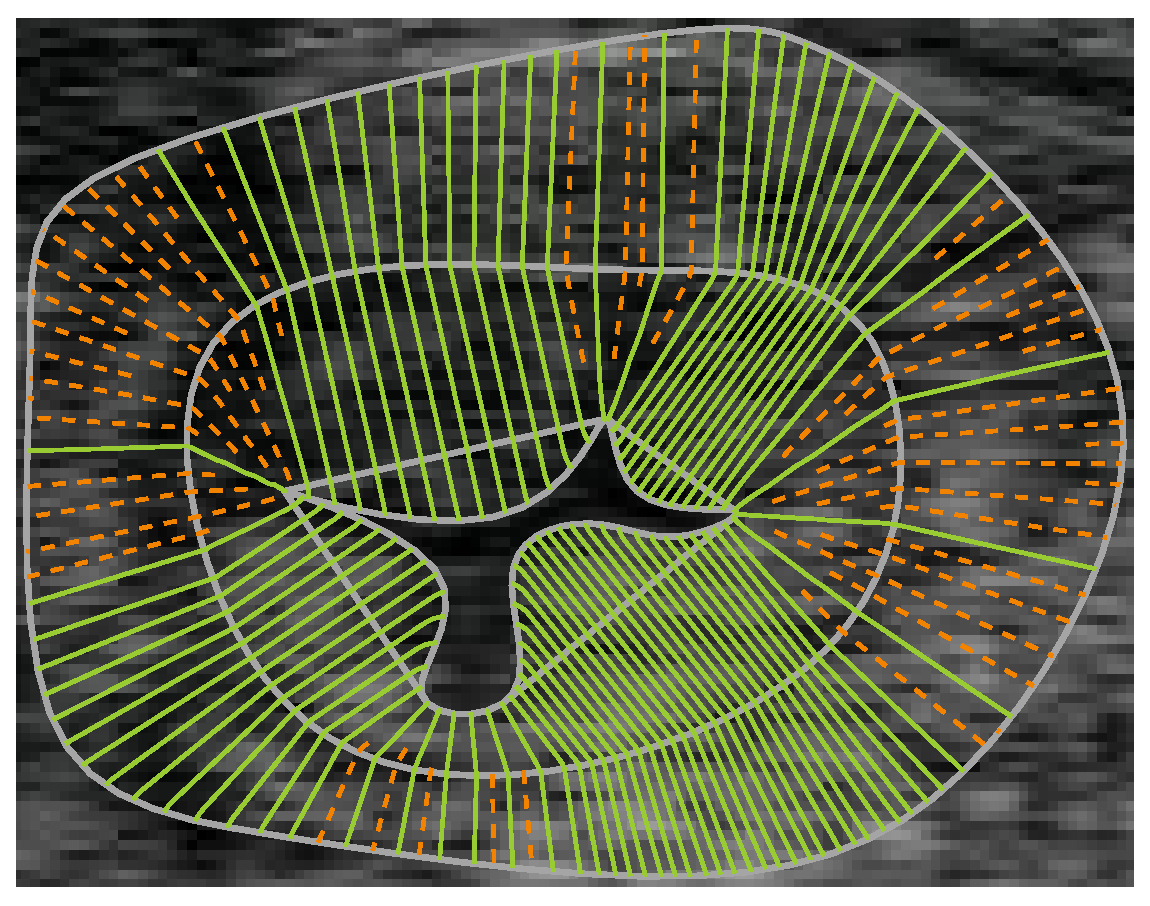
\includegraphics[width=5.5cm]{pics/rreal4}}
  \centerline{(c)}\medskip
\end{minipage}
\hfill
\begin{minipage}[b]{.33\linewidth}
  \centering
  \centerline{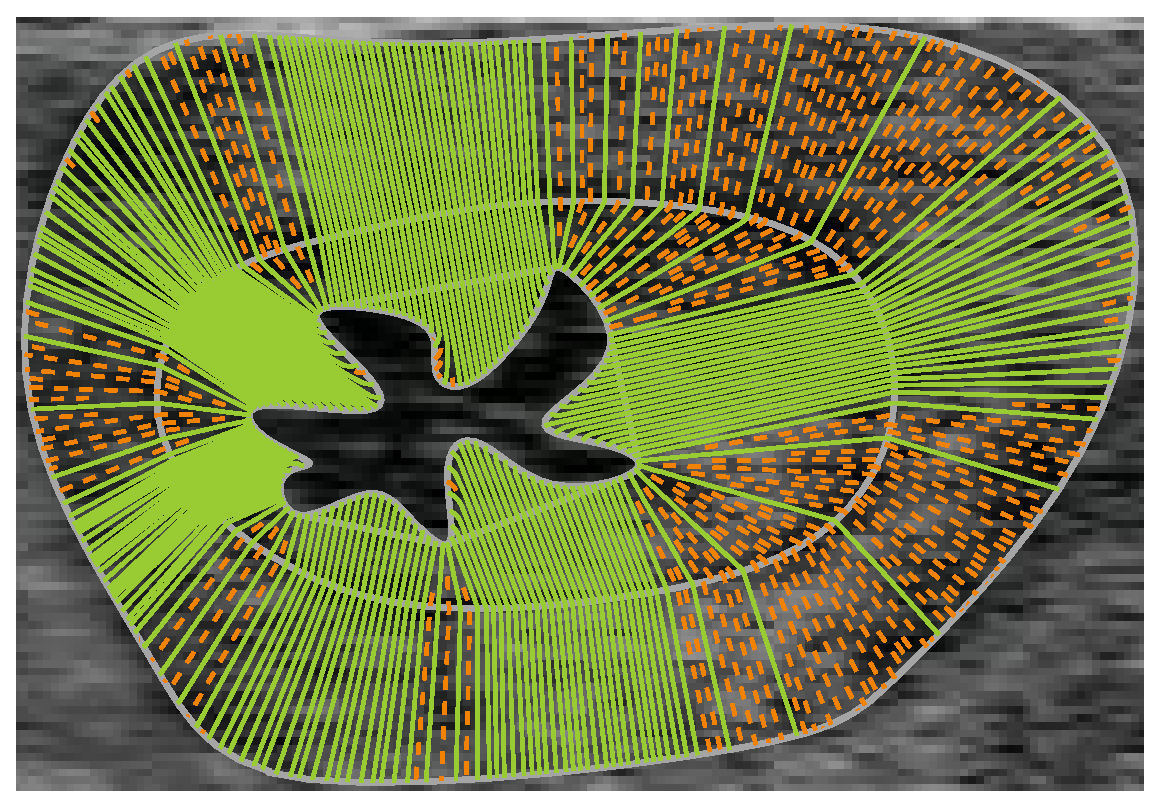
\includegraphics[width=6.2cm]{pics/rreal3}}
  \centerline{(e)}\medskip
\end{minipage}
\hfill
\begin{minipage}[b]{.33\linewidth}
  \centering
  \centerline{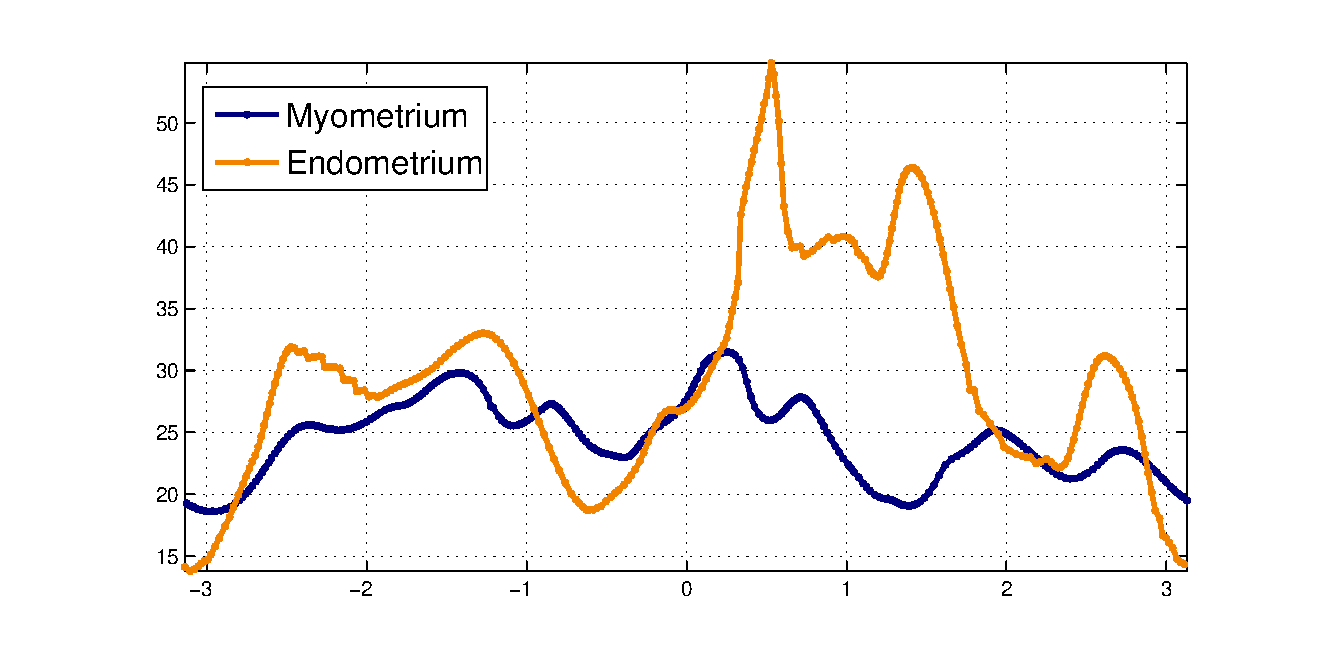
\includegraphics[width=6.5cm]{pics/realWidth}}
  \centerline{(b)}\medskip
\end{minipage}
\hfill
\begin{minipage}[b]{.33\linewidth}
  \centering
  \centerline{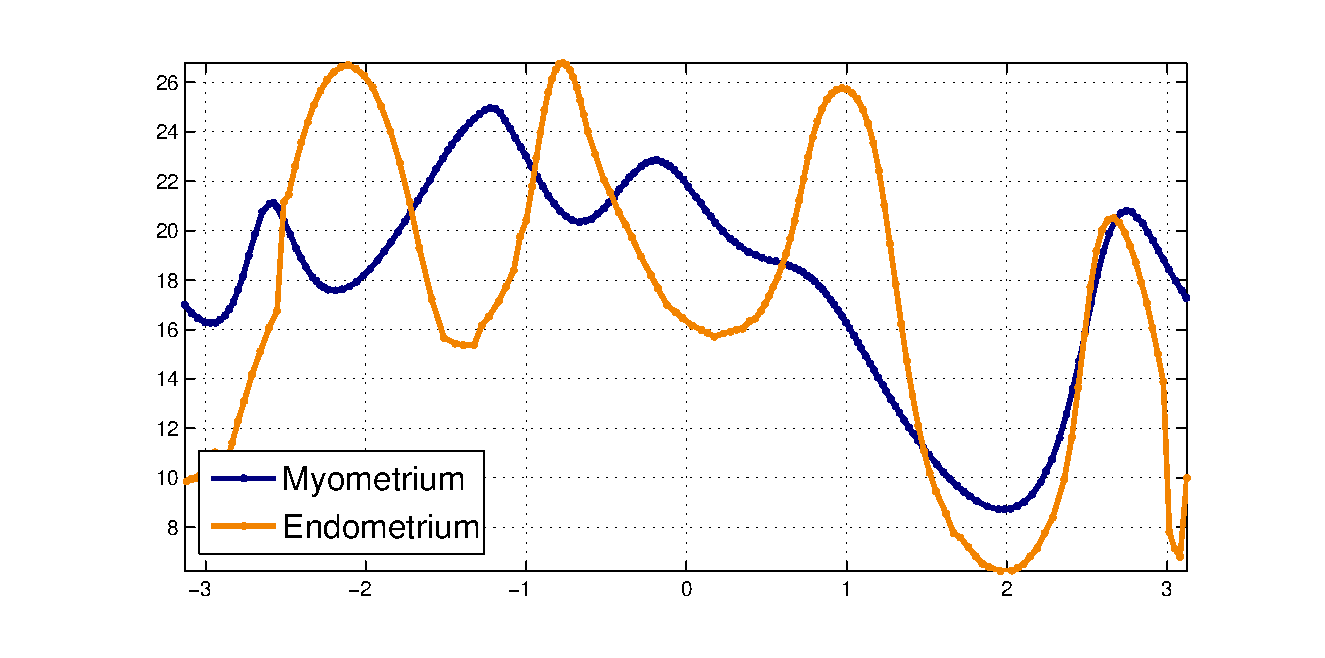
\includegraphics[width=6.5cm]{pics/realWidth4}}
  \centerline{(d)}\medskip
\end{minipage}
\hfill
\begin{minipage}[b]{.33\linewidth}
  \centering
  \centerline{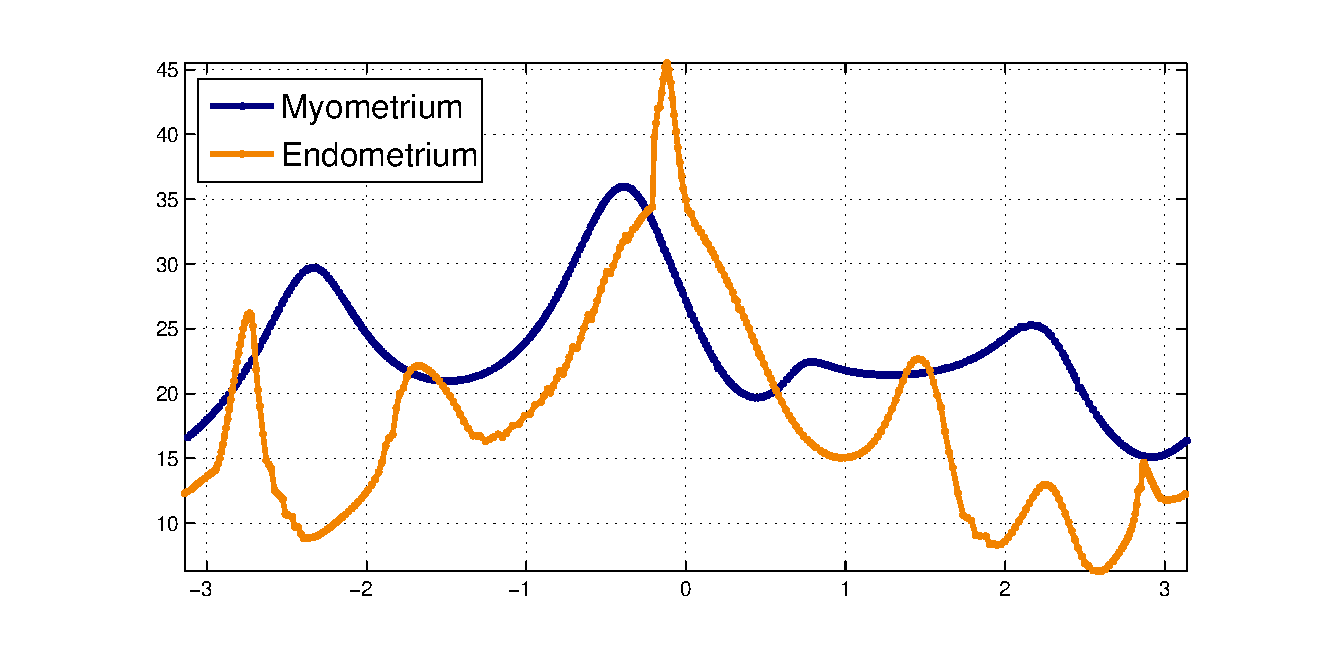
\includegraphics[width=6.5cm]{pics/realWidth3}}
  \centerline{(f)}\medskip
\end{minipage}
\vspace{-15pt}
\caption{Results on real images. Images shows three different real situations. In (a), (c) and (e) is shown the path traveled by points of curves during the evolution, and in (b), (d) and (f) their respective thickness profiles obtained. The blue line corresponds to the thickness between $\Gamma_1$ and $\Gamma_2$, and the orange line corresponds to the thickness between $\Gamma_2$ and $\Gamma_3$.}
\label{fig:real}
\end{figure*}

\subsection{Feature extraction and classification}
\label{ssec:clasification}
The algorithm was applied to a database tagged by the expert, knowing which cows has sub-clinical endometritis. In a preliminary study of the problem the thickness profile obtained for each image was used to obtain some descriptors in order to perform an automatic supervised classification in two classes: cattle with or without endometritis. The extracted features try to simulate what the expert analyzes to diagnose: maximum thickness of endometrium normalized by endometrium area and maximum thickness of myometrium with and without the area normalization.

Performing a feature selection using a wrapper method and classification with multilayer perceptron, we obtained results that, although preliminary, seems to be very promissory. Using a 6-fold cross validation we were able to correctly classify 91.67\% of instances, with a recall of 91.7\% and a precision of 92.9\%. This results are showing that the features obtained from the thickness profile, which could not be extracted using other measures such as euclidean distance, can play an important role in detecting sub-clinical endometritis.

\section{Conclusion}
\label{sec:conc}
In this work we present an algorithm to measure the thickness of a
region delimited by two closed curves, without any regularity
assumptions on the curves. The curves are sampled according to
curvature and the algorithm is based on the normal evolution with
constant velocity. Mechanisms of
creating and combining points during evolution were designed and
implemented, ensuring a good representation of the curve in each
step. To deal with the ``irregularity'', meaning the high variation of
curvature of a curve, the convex hull is considered as an auxiliary
curve and the evolution is performed in two steps: evolving from the
convex hull to the origin curve and evolving from the convex hull to
the target curve. This algorithm leads to an intuitive thickness
definition, and an entire thickness profile is obtained. When defining
the thickness, the correspondence between the curves is not clear in
other methods, but this algorithm finds a reasonable correspondence, resolving an entire mapping between curves.

The algorithm was applied to a particular problem, where the goal is to measure the thickness of a muscle of cattle uterus. This thickness appears to be very relevant to help the detection of a sub-clinical uterine disease: endometritis. Some descriptors were extracted from the thickness profile, and a simple classification system was implemented in order to classify sick cows. The results are very promissory, giving good prospects for automatic detection.

\subsection{Future work}
\label{ssec:future}
As future work we plan to explore in extracting better descriptors from the thickness profile and obtain other descriptors from the ultrasonographic images, such as texture or shape descriptors, in order to obtain a more accurate classification. Also we plan to enlarge the database.

\section{Acknowledgments}
The author would like to thank Gregory Randall, PhD., Dra.~Ana Meikle,
PhD. and Dra.~Isabel Pereira for their suggestions and fruitful
discussions. This work was partially funded by project ANII
FMV~2\_2011\_1\_7376.

\bibliographystyle{IEEEbib}
\bibliography{refs}

\balance

\end{document}

% To start a new column (but not a new page) and help balance the last-page
% column length use \vfill\pagebreak.
% -------------------------------------------------------------------------
%\vfill
%\pagebreak

% Below is an example of how to insert images. Delete the ``\vspace'' line,
% uncomment the preceding line ``\centerline...'' and replace ``imageX.ps''
% with a suitable PostScript file name.
% -------------------------------------------------------------------------
\begin{figure}[t]

\begin{minipage}[b]{1.0\linewidth}
  \centering
  \centerline{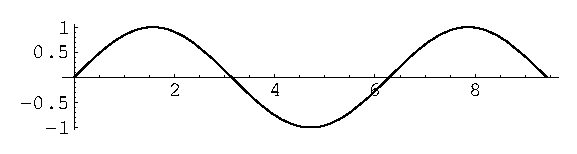
\includegraphics[width=8.5cm]{pics/image1}}
%  \vspace{2.0cm}
  \centerline{(a) Result 1}\medskip
\end{minipage}
%
\begin{minipage}[b]{.48\linewidth}
  \centering
  \centerline{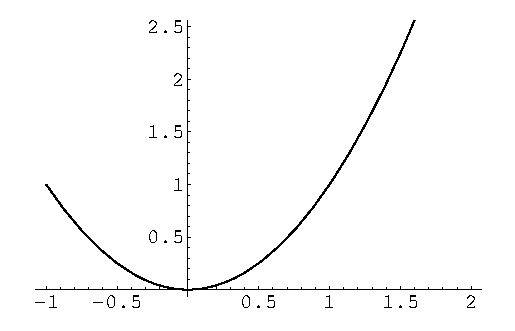
\includegraphics[width=4.0cm]{pics/image3}}
%  \vspace{1.5cm}
  \centerline{(b) Results 3}\medskip
\end{minipage}
\hfill
\begin{minipage}[b]{0.48\linewidth}
  \centering
  \centerline{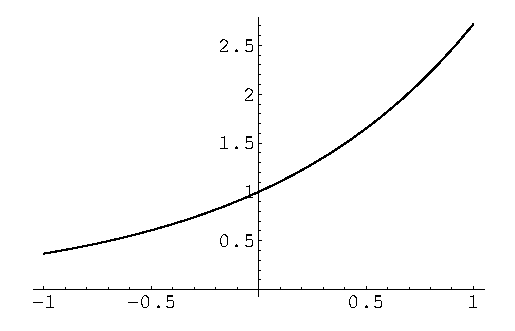
\includegraphics[width=4.0cm]{pics/image4}}
%  \vspace{1.5cm}
  \centerline{(c) Result 4}\medskip
\end{minipage}
%
\caption{Example of placing a figure with experimental results.}
\label{fig:res}
%
\end{figure}
